\documentclass[reprint,aps,prl,twocolumn,superscriptaddress,groupedaddress]{revtex4-2}
\usepackage{CJKutf8}
\usepackage[utf8]{inputenc}


\usepackage[final]{graphicx}
\usepackage[hidelinks]{hyperref}
\usepackage{bm,physics,amsmath,amssymb,xcolor}
\usepackage[normalem]{ulem}

\usepackage{centernot}
\usepackage{braket}
\usepackage{tabularx}
\usepackage{booktabs}
\usepackage{pifont}
\usepackage{colortbl}
\usepackage{amsthm}
\usepackage{soul}
\usepackage{epsfig}

\setcounter{secnumdepth}{4}
\usepackage{titlesec}

\newcommand{\eomo}{$E_1$-$M_1$}
\newcommand{\eoet}{$E_1$-$E_2$}
\newcommand{\etet}{$E_2$-$E_2$}
\newtheorem{theorem}{Theorem}
\newtheorem*{remark}{Theorem}
\definecolor{CL_Yellow}{HTML}{E69E5B}
\colorlet{LightYellow}{CL_Yellow!25}
\definecolor{CL_Pink}{HTML}{9E5BE6}
\colorlet{LightPink}{CL_Pink!25}
\definecolor{CL_Green}{HTML}{9EE65B}
\colorlet{LightBlue}{CL_Green!25}
\newcommand{\cg}[3]{C^{#1}_{#2;#3}}
\newcommand{\ii}{\mathrm{i}}

\newcommand{\correction}[2]{\textcolor{red}{\sout{#1}} \textcolor{blue}{#2}}
\newcommand{\hide}[1]{}

\usepackage{printlen}
\makeatletter
\edef\textFontName{\fontname\csname
  \f@encoding/\f@family/\f@series/\f@shape/\f@size\endcsname}
\edef\mathFontName{\fontname\textfont0}
\edef\mathLetterFontName{\fontname\textfont1}
\makeatother
\newcommand{\printsizes}{
    \uselengthunit{in}~\\
    textwidth: \printlength{\textwidth}\\
    linewidth: \printlength{\linewidth}\\
    text height: \printlength{\textheight}\\
    font name: \textFontName \\
    font size: \the\fontdimen6\font\relax
}
\begin{document}
\begin{CJK*}{UTF8}{gbsn}
\title{振转螺旋二色性的自下而上分析}
\author{Mateja Hrast}
\email[]{mateja.hrast@ist.ac.at}
\affiliation{奥地利科学技术研究所(ISTA),Am Campus 1, 3400 克洛斯特新堡,奥地利}
\author{Georgios M. Koutentakis}
\email{georgios.koutentakis@ist.ac.at}
\affiliation{奥地利科学技术研究所(ISTA),Am Campus 1, 3400 克洛斯特新堡,奥地利}
\author{Mikhail Maslov}
\email{mikhail.maslov@ist.ac.at}
\affiliation{奥地利科学技术研究所(ISTA),Am Campus 1, 3400 克洛斯特新堡,奥地利}
\author{Mikhail Lemeshko}
\email{mikhail.lemeshko@ist.ac.at}
\affiliation{奥地利科学技术研究所(ISTA),Am Campus 1, 3400 克洛斯特新堡,奥地利}
\date{\today}
\begin{abstract}
螺旋二色性(Helical Dichroism, HD)是一种利用光轨道角动量(Orbital Angular Momentum, OAM)解析分子手性的新兴方法。本研究突破传统理论对HD的假设,基于分子对称性与旋转本征态构建了严格的HD分析理论框架。我们推导出旋转选择规则,明确证明即使对于无远场OAM的光束,HD现象也仅源于光的自旋-轨道耦合作用。该发现完善了观测HD的条件,不仅为先前实验结果提供理论解释,更为未来基于结构光的手性传感设计提供了重要指导。
\end{abstract}
\maketitle
许多具有生物和化学重要性的分子以手性对形式存在——这两种互为镜像却无法重叠的版本称为对映体。分离对映体的能力对于制药和农用化学品工业至关重要\cite{MAIER2001}。甲基苯丙胺分子最能说明这一点:其R-对映体是有效的鼻充血缓解剂,而S-对映体则是导致成瘾流行的精神活性药物~\cite{barkholtz2023}。高度的经济相关性推动了对不对称合成手性分子的研究,例如通过立体选择性或生物催化,或使用手性辅助剂\cite{Brown1989}。然而,这些先进合成技术需要进一步优化,并通过立体选择性过程评估对映体纯度。这一关键步骤目前仍面临技术挑战,现有化学方法各自存在局限性,包括高成本、耗时、适用性有限和可靠性不足等问题\cite{qian2023}。本文从化学物理的视角提出替代方案,旨在通过光-物质相互作用评估对映体纯度。得益于光学物理的快速发展\cite{Koch2019},这种方法为手性识别提供了一条经济高效且高度可控的途径。

数十年来,左旋和右旋圆偏振光吸收差异(即圆二色性CD)\cite{deutsche1970,Holzwarth1974}已被用于手性介质的光谱分析\cite{Miles2021}。但圆二色性依赖于光的自旋角动量这一有限资源。与此同时,Allen等人的开创性光学工作\cite{Allen1992}证明光除了自旋外还具有轨道角动量(OAM)。与自旋不同,光束携带的OAM量子数原则上没有上限。携带OAM的光束具有螺旋波前结构,这种手性特征可能与物质的手性相匹配,为立体选择性应用带来前所未有的可能性。

这种设想催生了利用OAM诱导过程检测对映体纯度的具体方案,特别是螺旋二色性(HD)\cite{ANDREWS2004,Ye2019,Li2021},其被认为是对CD的重要改进\cite{Ye2019,Li2021}。Forbes和Andrews的基础理论研究\cite{Forbes2018,Forbes2019,Forbes2021}为HD奠定了理论基础,他们系统分析了光-物质相互作用多极展开项的对称性,指出电偶极-磁偶极(\eomo)、电偶极-电四极(\eoet)和电四极-电四极(\etet)项可作为手性鉴别因子。他们推导了\eoet跃迁振幅与分子多极矩的关系表达式,但未尝试用分子转动态来评估这些多极矩。实验方面,早期尝试未观察到HD信号\cite{Araoka2005,Loeffler2011},但近期实验声称实现了观测\cite{Rusak2019,Zhang2020,Rouxel2022,Begin2023,Jain2023}。然而这些实验装置极其复杂,尽管理论认为强聚焦是必要条件\cite{Forbes2019},但尚未有研究阐明观测到的二色性起源。

本研究通过揭示转动振动光谱中产生HD的条件填补了这一空白。我们首先概述基于分子多极矩的手性检测方法,推导观测\eoet二色性的对称性要求。利用新近发展的分子-光相互作用哈密顿量\cite{Maslov2024,Maslov_Thesis},我们推导了\eoet项诱导的转动振动跃迁选择定则。通过分析这些定则,证明傍轴拉盖尔-高斯(LG)光束无法产生真正的HD(即源于OAM转移的HD)。特别地,强聚焦至关重要——因为光的自旋-轨道耦合(SOC)\cite{Bliokh2015}能使手性分子获得OAM,产生傍轴近似下不存在的HD贡献。我们还证明,即使不携带远场OAM的高斯光束在强聚焦条件下也能产生HD信号。这些发现完善了转动振动光谱中HD的理论基础,为未来利用结构光进行实验设计和立体选择性技术开发提供了指导。

现有多种对映体敏感方法基于分子多极矩分析。标准手性检测方法——(振动)圆二色性涉及\eomo项,已有详尽研究\cite{Stephens1985,BUCKINGHAM1987,Mun2019,Lovesey2019}。其原理在于:手性分子的电偶极矩在镜像反射下会改变符号(作为真矢量),而磁偶极矩(赝矢量)保持不变。两者共存表明分子缺乏镜面对称性(严格说是非真旋转轴),即具有手性。该方法要求分子对称性允许至少一个非零偶极矩,因此能检测多种对称群的手性分子。但源于\eomo项的二色性仅取决于场强,这使得其他可通过场结构增强二色性的机制更具吸引力。

相位敏感微波三波混频技术\cite{Patterson2013,Patterson2013PRL}即为一例,其利用偶极矩乘积$d_xd_yd_z\neq 0$作为手性判据\cite{Patterson2013,Ordonez2018,Ayuso2022}。对称性分析表明,仅完全不对称($C_1$)手性分子符合此条件。我们研究探索了另一方向——源于分子电偶极矩和电四极矩的手性条件。\eoet项诱导的二色性可通过适当结构的光场增强,这使其成为未来对映体敏感技术的理想候选。近期研究还提出磁偶极-磁四极($M_1$-$M_2$)耦合可作为HD来源,其对称性与\eoet项等效\cite{Ji2024}。但此类高阶项(如\etet)由于多极展开中跃迁概率较低,实验检测难度较大。\\
本文剩余部分将重点研究源自\eoet 项的二向色性特征。基于简单的点电荷模型,我们推导出以下条件(证明见补充材料\footnote{参见补充材料,其中包含参考文献\cite{Maslov2024,Maslov_Thesis,Lax1975,Bliokh2015,Bliokh2023}}):\\
\textit{若在主轴坐标系中,对于不同的$\mu, \nu, \rho \in \{x,y,z\}$坐标,偶极矩与四极矩的乘积$d_{\mu}Q_{\nu \rho} \neq 0$,则该分子具有手性。}\\
该条件迄今一直与螺旋二向色性(HD)相关联\cite{ANDREWS2004,Forbes2018}。然而本研究表明,即便光场未向分子内自由度传递轨道角动量(OAM),该条件仍可导致鉴别效应。本文中HD特指伴随OAM转移的二向色性效应,而不涉及OAM转移的效应(即便使用携带OAM的光束)则称为圆二色性(CD)。

表~\ref{tab:chiral_multipole_dofs}总结了\eoet 项可诱导二向色性的手性点群。在纯转动光谱中,仅需考虑分子的永久多极矩;而振动-转动光谱中,振动跃迁会改变分子态的对称性,因此需结合终态振动能级不可约表示$V$的变换特性进行分析,这使得更多手性群组可被检测。该表列出了各手性点群中呈现二向色性的$V$表示。
\begin{table}[ht!]
    \centering
    \caption{所有可能手性点群的旋转光谱与旋转振动光谱中的\eoet~手性特征。对于旋转振动光谱,我们给出了与非零手性特征相关联的振动模式的不可约表示。}
     \setlength\tabcolsep{3pt}
\begin{tabular}{p{70pt} | c c c c c c c c c c}
\toprule
     Point group     & $C_1$ & $C_2$ & $C_{n\geq 3}$ & $D_2$ & $D_{n\geq 3}$ & $T$ & $O$ & $I$ \\ \midrule
     Rotational      & \textcolor{black}{\ding{52}} & \textcolor{black}{\ding{52}}& \textcolor{red}{\ding{56}}  & \textcolor{red}{\ding{56}}  & \textcolor{red}{\ding{56}}  & \textcolor{red}{\ding{56}}  & \textcolor{red}{\ding{56}}  & \textcolor{red}{\ding{56}} \\
     Ro-vibrational  & $A$ & $A$, $B$ & $E_1$ & $B_{1, 2, 3}$ & $E_1$ & $T$ & \textcolor{red}{\ding{56}} & \textcolor{red}{\ding{56}} \\
     \bottomrule
\end{tabular}
     \label{tab:chiral_multipole_dofs}
 \end{table}
如表\ref{tab:chiral_multipole_dofs}所示,\eoet项仅能通过保持分子对称性的跃迁(纯转动及平凡表示$A$的振动-转动)识别$C_1$和$C_2$对称性的手性分子。鉴于已知手性分子多为$C_1$对称(即不对称陀螺分子)\cite{Bernath},本文研究范围限定于此。

不对称陀螺转子哈密顿量的本征态以转动基矢$\ket{J,M,K}$\cite{Bernath}表示为:
\begin{equation}
    \ket{J_{N_p,N_o}(M)}=\sum_KC_K\ket{J,M,K}.
    \label{basisChange}
\end{equation}
其中$J$为总角动量量子数,$M$和$K$分别为${\bm J}$在实验室量子化轴和本体主轴系上的投影。不对称陀螺指标$N_p$与$N_o$是纯扁长/扁球解中$K$的极限值,并非好量子数。由于量子数$J$和$M$不受基变换\eqref{basisChange}影响,我们进一步推导转动基矢$| J, M, K \rangle$内电偶极($E_1$)与电四极($E_2$)跃迁的选择定则。

初态$i=\ket{J,M,K}$至末态$f=\ket{J,M',K'}$的分子转动态跃迁速率可通过文献\cite{Maslov2024,Maslov_Thesis}中的光-物质相互作用哈密顿量计算,其跃迁振幅为:
\begin{equation}
    \mathcal{M}_{i\to f}=\sum_{lm\mu}\mathcal{I}^{\text{vib}; l,\mu}\,\mathcal{I}^{\text{CM}; l,m}\,\mathcal{I}^{\text{rot}; l,m,\mu,\sigma}_{J,M,K,J,M',K'}\,,
    \label{eq_transition_matrix}
\end{equation}
式中$l=0$和$l=1$分别对应偶极与四极跃迁,$m = 0, \pm 1, \dots, \pm l$为转移至分子的OAM,$\mu = 0, \pm 1, \dots, \pm (l+1)$遍历球基下所选多极矩的所有分量,$\sigma =0, \pm 1$表示光的偏振分量。振动项$\mathcal{I}^{\text{vib}; l,\mu}$与质心项$\mathcal{I}^{\text{CM}; l,m}$分别参数化分子与光场特性。本文重点关注支配角动量选择定则的转动跃迁振幅$\mathcal{I}^{\text{rot};l,m,\mu,\sigma}_{J,M,K,J,M',K'}$,其总结于表~\ref{SelectionRules}。
\begin{table}[ht!]
    \centering
    \begin{tabular}{c c}\hline
    \toprule
        \textbf{$E_1$ transition} & \textbf{$E_2$ transition}  \\
        \midrule
        $\Delta J\leq 1$ &  $\Delta J\leq 2$ \\
        $\Delta M=-\sigma$ & $\Delta M=m-\sigma$ \\
        $\Delta K=\pm\mu$ & $\Delta K=\pm\mu$ \\
        $J=0\not\to J'=0$ &  (see \cite{Note1}\\
        $\ket{J,0,K}\not\to\ket{J,0,K'}$ &  for details)\\
    \bottomrule
\hline
    \end{tabular}
    \caption{电偶极 ($E_1$) 与四极 ($E_2$) 跃迁在转动态 $\ket{J,M,K}$ 之间的选择定则。关于禁戒跃迁的详细说明参见 \cite{Note1}。}
    \label{SelectionRules}
\end{table}
可以证明$\mathcal{I}^{\rm rot; l, m, \mu, \sigma}_{J, M, K, J', M', K'} \propto C^{J',M'}_{l+1, m-\sigma; J, M}$ \cite{Maslov2024,Maslov_Thesis},其中$C^{J, M}_{j_1, m_1, j_2, m_2}$为克莱布什-戈尔丹系数(推导过程见补充材料\cite{Note1})。要实现电偶极-电四极(\eoet)跃迁,所选态之间必须同时允许$E_1$($l=m=0$)和$E_2$($l = 1$,$m = 0, \pm 1$)跃迁。对于具有确定偏振$\sigma$的光束,这仅可能发生在$m = 0$的光场分量中——该分量不携带轨道角动量(见表~\ref{SelectionRules})。由此我们得到本工作的首个关键结论:源于傍轴光束\eoet~项的二色性不应与螺旋二色性(HD)关联,因为此时分子未获得轨道角动量。此外,这种二色性甚至在平面波情形下也存在,因此与光场结构或螺旋性完全无关。

这引出一个问题:当发生轨道角动量转移时,\eoet~项能否产生HD?下文将证明,在非傍轴光束情形下可以实现这种机制。图~\ref{fig:gridJ1}展示了不对称陀螺分子转动态之间允许的偶极跃迁(红色方框)与四极跃迁(蓝色方框)。为清晰起见,图中仅显示部分本征态,完整图谱($J\leq 2$)见\cite{Note1},但其定性特征与此一致。

\begin{figure}[ht!]
    \centering
    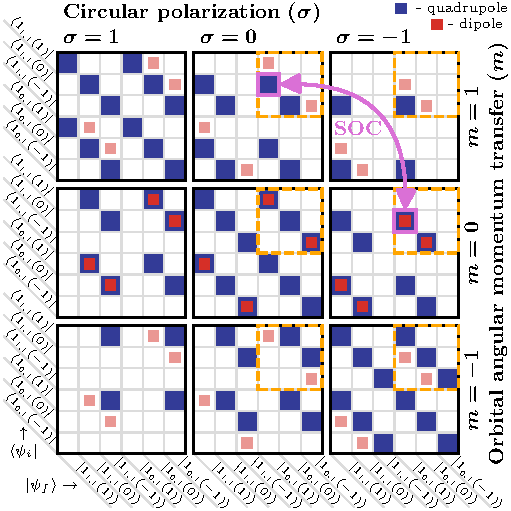
\includegraphics[width=\linewidth]{Figure1.pdf}
    \caption{不对称陀螺哈密顿量本征态之间允许的偶极跃迁(红色方块)与四极跃迁(蓝色方块)。各子图列表示光束的不同圆偏振态,子图行表示光束可传递给分子内转动的轨道角动量数值。紫色圆圈展示了自旋-轨道耦合产生伴随轨道角动量转移的\eoet 项的实例。橙色方块标明了实验中会叠加的跃迁(如图\ref{fig:profiles}所示)。}
    \label{fig:gridJ1}
\end{figure}
图~\ref{fig:gridJ1}的三列对应不同光束偏振态,三行对应不同轨道角动量转移量子数$m$。如文献\cite{Maslov2024,Maslov_Thesis}所示,电偶极跃迁不转移轨道角动量,故仅出现在$m=0$行(但为便于比较,我们在$m=\pm 1$行也予以标注)。相反,电四极跃迁可转移最多一个轨道角动量量子($m=0,\pm 1$)。任何非平面波束通常包含这三行的贡献,但其相对权重取决于具体光束结构。

我们首先关注红蓝方框标记的态对——它们同时存在偶极和四极跃迁。这些跃迁全部出现在$m=0$行,即不发生轨道角动量转移的情形。这验证了表~\ref{SelectionRules}的结论,表明对于具有确定$\sigma$的光束,\eoet~项无法产生HD,仅是对圆二色性(CD)的额外贡献。

然而,轨道角动量($m$)与自旋($\sigma$)的明确分离仅适用于傍轴光束。实际上,任何类型的光自旋-轨道耦合(SOC)都会导致不同$\sigma$分量的混合\cite{Bliokh2015,Bliokh2023}。这意味着图~\ref{fig:gridJ1}中不同面板的项可共同驱动同一跃迁。例如,紫色方框对应的\eoet~项将同时包含偶极跃迁($m=0$,$\sigma=-1$)和四极跃迁($m=0$,$\sigma=-1$及$m=1$,$\sigma=0$):$| 1_{0,1}(1) \rangle \to | 1_{1,1}(0) \rangle$。偶极矩项与$m=-1$四极分量的耦合使分子能够感知轨道角动量的影响。

实现此类跃迁所需的光自旋-轨道耦合可通过紧聚焦拉盖尔-高斯光束实现\cite{Loeffler2011,Forbes2021nonparaxial,Forbes2021longitudinal}。我们采用一阶非傍轴近似描述光束\cite{Lax1975}(详见\cite{Note1}),并利用文献\cite{Maslov2024,Maslov_Thesis}的相互作用哈密顿量计算图~\ref{fig:gridJ1}虚线方框态间的空间分辨矩阵元。参数设置为:四极跃迁矩$Q_{xy}=0.5d_z\lambda$($d_z$为偶极跃迁矩,$\lambda$为波长),焦斑半径$\omega_0=0.2\lambda$,离焦距离$z=\lambda$($z$为传播方向),拉盖尔-高斯光束的拓扑电荷$L_{\rm beam}=1$,偏振$\sigma=-1$。对映异构体通过分子固定(惯性)$xy$平面的反射描述。已有明确研究\cite{Buckingham1971, Power1975}表明观测\eoet~相互作用需要各向异性,因此任何HD实验都需要$M$态分辨。$M$态分辨的信号分布如图~\ref{fig:profiles}所示。

\begin{figure}[t!]
    \centering
    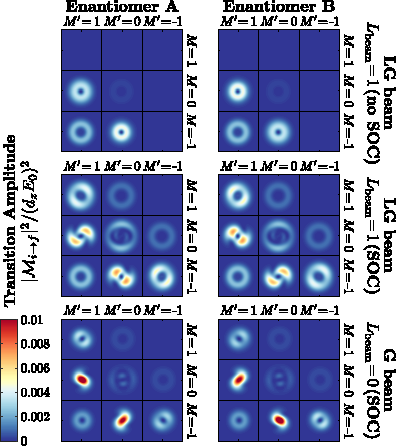
\includegraphics[width=1.0\columnwidth]{Figure2.pdf}
    \caption{对映异构体在拉盖尔-高斯光束耦合下$\bra{1_{1,1}(M)}$到$\ket{1_{0,1}(M')}$跃迁的信号剖面(上:无自旋轨道耦合;中:有自旋轨道耦合)及高斯光束耦合下自旋轨道耦合作用的信号剖面(下)。}
    \label{fig:profiles}
\end{figure}
首先注意到,除非$d_zQ_{xy}^*$存在虚部${\rm Im}[d_zQ_{xy}^*]$,否则所有分布曲线的积分值相等。该虚部会导致总吸收水平的二色性,这是已知的振动CD来源,其仅取决于分子内部参数而与电场结构无关(见\cite{Buckingham1971})。由此得出结论:仅通过光吸收强度无法检测HD,必须借助吸收分布的空间分辨\cite{Loeffler2011}。

若无光自旋-轨道耦合,两个对映体间仅存在$M=0\to M'=1$与$M=-1\to M'=0$分布强度的差异(图~\ref{fig:profiles}顶行)。该二色性源于光束的$m=0$分量——即图~\ref{fig:gridJ1}中$\sigma=-1$、$m=0$面板虚线框内的红蓝方框。因此这是另一种空间分辨振动CD来源,因未发生轨道角动量转移。

焦场引入的光自旋-轨道耦合导致吸收分布中出现新的对映体区分效应(图~\ref{fig:profiles}中行)。首先,$M=-1\to M'=0$与$M=0\to M'=1$跃迁的吸收存在显著差异。该信号源自图~\ref{fig:gridJ1}虚线方框内偶极与四极跃迁的耦合。这种差异源于涡旋光束与手性分子的相对螺旋性,并涉及轨道角动量转移,因此可视为真正的HD。
接下来,$M=1\to M'=1$与$M=-1\to M'=-1$的谱线轮廓也存在差异。这源于虚线框中$\sigma=0$的偶极跃迁(图~\ref{fig:gridJ1})与$m=-1$、$\sigma=-1$方框中四极跃迁的耦合作用。因此,这也属于螺旋二色性(HD)现象。总体而言,自旋轨道耦合(SOC)光作用下的二色性信号强度比无耦合情形高出一个数量级。

图\ref{fig:profiles}最下行表明,在SOC情形下,渐近极限中无需使用携带轨道角动量(OAM)的光束。事实上,紧聚焦高斯光束同样能观测到HD效应。这是因为焦场会呈现为方位角电荷$\sigma$的拉盖尔-高斯(LG)模式。实际上,紧聚焦的线偏振光束也会产生类似二色性,因为其内部两个圆偏振分量会通过SOC发生耦合。这说明入射光束的OAM或自旋都不是观测HD的必要条件,真正的关键因素在于SOC。

需注意的是,由于光场的SOC效应,传递给分子的角动量类型难以明确区分,这使得我们无法简单地将产生的二色性归类为圆二色性(CD)或螺旋二色性(HD)。我们的工作通过量子数$m$和$\sigma$(见图~\ref{fig:profiles})明确了OAM与自旋的吸收通道,为解决该问题提供了途径。

综上所述,我们证明了傍轴OAM光束无法产生HD,因为这些条件下观测到的二色性都会退化为标准CD。真正的HD——即直接与OAM传递相关的二色性——需要光场的自旋轨道耦合,如紧聚焦光束所展现的那样。引人注目的是,纯高斯模式在充分聚焦后也能展现真正的HD效应,尽管其在远场中并不携带OAM。这些发现阐明了结构光实验中HD的起源,并提示此前关于HD的测量结果可能需要仔细复核以确认OAM转移的存在。特别是,那些未能观测到二色性的研究,要么主要探测偶极级相互作用\cite{Araoka2005},要么因信号平均化而丢失二色性特征\cite{Loeffler2011}。而成功检测到二色性的研究,则同时利用了四极场相互作用和紧聚焦光束\cite{Rusak2019,Rouxel2022,Begin2023,Jain2023}。

本文建立的框架为设计基于光场空间结构的手性敏感光谱学和对映体分离方法提供了路线图~\cite{Leibscher2022}。\\
\begin{acknowledgments}
本研究全部或部分由奥地利科学基金(FWF)资助[项目编号:10.55776/F1004]。
\end{acknowledgments}
\bibliography{bibliography}
\end{CJK*}
\end{document}
